\documentclass[12pt, openany]{report}

\usepackage[utf8]{inputenc}
\usepackage[T1]{fontenc}
\usepackage[a4paper,left=2cm,right=2cm,top=2cm,bottom=2cm,headheight = 15pt]{geometry}
\usepackage{libertine}
\usepackage[pdftex]{graphicx}
\usepackage{totpages}
\usepackage[hidelinks]{hyperref}

\usepackage{helvet}
\renewcommand{\familydefault}{\sfdefault}
\usepackage[english, french]{babel}
\usepackage{subcaption}

\usepackage{setspace}
\onehalfspacing

% Change l'espacement entre deux paragraphes
\setlength{\parskip}{18pt}

% Liste à puces
\frenchbsetup{StandardLists=true}

% Édite style sous-titre figure et tableau
\usepackage[font=it]{caption}

% Change l'en-tête et le pied de page pour tout le document
\usepackage{fancyhdr}
\pagestyle{fancy}

\renewcommand{\chaptermark}[1]{\markboth{\thechapter.\ #1}{}}
\renewcommand{\sectionmark}[1]{\markright{\thesection.\ #1}}

\renewcommand{\headrulewidth}{0.5pt} 
\fancyhead[L]{\bfseries\leftmark}
\fancyhead[C]{}
\fancyhead[R]{\rightmark}

\renewcommand{\footrulewidth}{0.5pt}
\fancyfoot[L]{\textbf{Tugdual Le Pen}}
\fancyfoot[C]{}
\fancyfoot[R]{\thepage\ / \ref{TotPages}}

\fancypagestyle{plain}{ %
    \fancyhf{} % remove everything

    \renewcommand{\headrulewidth}{0pt} 
    \renewcommand{\footrulewidth}{0.5pt}
    \fancyfoot[L]{\textbf{Tugdual Le Pen}}
    \fancyfoot[C]{}
    \fancyfoot[R]{\thepage\ / \ref{TotPages}}
}

% Change le style des parties et sous partiess
\usepackage[explicit]{titlesec}
% change l'espacement au niveau du titre des chapitres
\titlespacing*{\chapter}
  {0pt}%  indent
  {0pt}% space before
  {12pt}% space after

\titlespacing*{\section}
  {0.6cm}%  indent
  {0pt}% space before
  {0pt}% space after

% Définie les couleurs utilisées dans le rapport
\usepackage{color}

\definecolor{darkblue}{rgb}{0.11, 0.30, 0.66}
\definecolor{lightblue}{rgb}{0.18, 0.42, 0.86}
\definecolor{gray}{rgb}{0.4,0.4,0.4}
\definecolor{black}{rgb}{0.0,0.0,0.0}
\definecolor{green}{rgb}{0.4, 0.8, 0.2}

%% Style Chapitre
% -------------------------------------------------------
% Avec numéro
\titleformat{\chapter}[hang] 
    {\fontsize{24pt}{0pt}\selectfont \bfseries}
    {\textcolor{darkblue} 
    {\thechapter. #1}}
    {0pt}
    {\huge}

% Sans numéro
\titleformat{name=\chapter,numberless}[hang] 
    {\fontsize{24pt}{0pt}\selectfont \bfseries}
    {\textcolor{darkblue} 
    {#1}}
    {0pt}
    {\huge}
% -------------------------------------------------------

%% Style Section
% -------------------------------------------------------
% Avec numéroté
\titleformat{\section}[hang]
    {\fontsize{16pt}{0pt}\selectfont \bfseries}
    {\textcolor{lightblue} 
    {\thesection.\ #1}}
    {10pt}
    {\Large}

% Sans numéro
\titleformat{name=\section,numberless}[display] 
    {\fontsize{16pt}{0pt}\selectfont \bfseries}
    {\textcolor{lightblue} 
    {\thechapter.\thesection #1}}
    {10pt}
    {\Large}
% -------------------------------------------------------

% Numérotation des chapitre en chiffre Romain
\renewcommand{\thechapter}{\Roman{chapter}}

% Créer commande pour lien url
\newcommand{\link}[1]{{\color{lightblue}\href{#1}{#1}}}

% Éviter les orphelin en début ou fin de page
\widowpenalty=10000 
\clubpenalty=10000 
\raggedbottom

% Nouvelle commande pour ajouter des commentaire sur le rapport
\newcommand{\comment}[1]{\emph{\color{green} \% #1}}



\begin{document}
\selectlanguage{french}
% Édite style sous-titre image et tableau
\makeatletter
\newcommand{\figcapfont}{\itshape} 
\newcommand{\tabcapfont}{\itshape}
\renewcommand{\fnum@figure}{\figcapfont Image \thefigure}
\renewcommand{\fnum@table}{\tabcapfont Tableau \thetable}
\makeatother

\begin{titlepage}
  \begin{center}

    % Logo Esir and Irisa
    % Author and supervisor
    \begin{minipage}{0.45\textwidth}
      \begin{flushleft} \large
        
\includegraphics[width=0.9\columnwidth]{datas/logo_esir.jpg}~\\
        \emph{Élève-ingénieur :}\\
        Tugdual Le Pen\\
        Imagerie Numérique\\
        2\up{ème} année du cursus ingénieur\\
        ~\\
        \emph{Tuteur universitaire :}\\
        Pierre Maurel\\
        Enseignant Chercheur
      \end{flushleft}
    \end{minipage}
    \begin{minipage}{0.45\textwidth}
      \begin{flushright} \large
        \vspace{19pt}
        
\includegraphics[width=0.9\columnwidth]{datas/logo_irisa.jpg}~\\~\\
        IRISA\\
        263 Avenue du Général Leclerc\\
        35000 RENNES - France\\
        contact@irisa.fr\\
        ~\\        
        \emph{Tuteur d'entreprise :}\\
        Olivier Le Meur\\
        Enseignant Chercheur\\
      \end{flushright}
    \end{minipage}

    \vspace{4cm}

    \textsc{\Huge \textbf{Étude et modèle prédictif de la saillance sur des œuvres d’art}}\\    

    \vfill

    % Bottom of the page
    \begin{minipage}{0.45\textwidth}
      \begin{flushleft}
        \vspace{0.5cm}
        {\large Année universitaire 2019 - 2020}
      \end{flushleft}
    \end{minipage}
    \begin{minipage}{0.45\textwidth}
      \begin{flushright}
        
\includegraphics[width=0.9\columnwidth]{datas/logo_univ.png}~\\
      \end{flushright}
    \end{minipage}

  \end{center}
\end{titlepage}

% Actualise le compteur de page
\clearpage
\setcounter{page}{2}

\addcontentsline{toc}{chapter}{Remerciements}
\chapter*{Remerciements}
\par
    Je tiens dans un premier temps à exprimer ma gratitude à l'IRISA et plus 
    particulièrement à l'équipe Percept pour m'avoir accueilli et considéré en 
    tant que collaborateur durant ces six mois de stage.

\par
    Je remercie mon tuteur Olivier Le Meur pour sa pédagogie, sa confiance et 
    son savoir-faire qui m'ont permis d'avancé sur mon projet serainement et 
    efficacement.

\par
    Merci également aux doctorants et ingénieurs de l'équipe Percept avec qui 
    j'ai pu échanger des bons moments et des conseils précieux pour le 
    développement de mon projet.
    
\par
    Je désire aussi aussi remercier les professeurs de l‘Ecole Supérieure 
    d'ingénieurs de Rennes, qui m’ont fourni les outils nécessaires au bon 
    déroulement de mon stage. Je tiens à remercier spécialement Pierre Maurel 
    mon professeur référent universitaire.

\par
    Enfin, pour conclure, je souhaiterais remercier toutes les personnes qui ont 
    participé de différentes façons à la réussite de mon stage.

\addcontentsline{toc}{chapter}{Résumé}
\chapter*{Résumé}
\par
    Pour valider ma 4\up{ème} année de mon cycle ingénieur en Technologie de 
    l'Information avec spécialité Imagerie Numérique, j'ai effectué un stage 
    d'une durée de six mois dans l'Institut de Recherche en Informatique et 
    Systèmes Aléatoires (IRISA). C'est un laboratoire de recherche impliqué dans 
    le domaine de l'informatique et des technologies de l'information. Il couvre 
    l'ensemble des thématiques de ces domaines, de l’architecture des 
    ordinateurs et des réseaux à l’intelligence artificielle en passant par le 
    génie logiciel, les systèmes distribués et la réalité virtuelle.

\par
    J'ai rejoint plus précisément l'équipe Percept (2018) qui est spécialisée 
    dans le comportement visuel de différentes populations. L'un des projets de 
    cette équipe est d'étudier la saillance dans les peintures. Notamment la capacité 
    de déterminer cette saillance automatiquement au moyen de machine learning.

\par
    Mon objectif est de participer à ce projet et mettre en place des 
    applications qui permettraient de montrer les possibiltés d'utilisations de 
    ce genre de programme.

\vspace{40pt}

\selectlanguage{english}
\color{gray}
\par
    To validate my 4\up{th} year of my engineer cycle specializing in Digital 
    Imaging, I did a six-month internship in the Research Institute in Computer 
    Science and Random Systems (IRISA). It is a research laboratory involved in 
    the field of computer science and information technology. It covers all the 
    themes of these fields, from the architecture of computers and networks to 
    artificial intelligence, including software engineering, distributed systems 
    and virtual reality. 

\par
    I joined the team Percept (2018) which specializes in the visual behavior of 
    different populations. One of the projects of this team is to study the 
    saliency in paintings. In particular the ability to determine this salience 
    automatically by means of machine learning. 

\par
    My objective is to participate in this project and set up applications which 
    allow us to show the possibilities of uses of this kind of program.

\selectlanguage{french}
\color{black}

% Renomme "Tables des matières" en "Sommaire"
\renewcommand{\contentsname}{Sommaire}
{\setlength{\parskip}{6pt}
\tableofcontents
}

\chapter{Introduction}

% rapide résumé contexte, explication du sujet et pk avoir choisi le stage

%Intro contexte
\par
La peinture et le mouvement du regard de l'Homme ont toujours eu un lien étroit. En effet chaque spectateur regardera un tableau d'une manière différente de son voisin parce que chaque individu a sa propre culture, son propre point de vue... Pourtant la structure d'une peinture amènera le spectateur à suivre un sens de lecture. Celui-ci sera généralement commun à tous les spectateurs. Par exemple un individu qui découvre le tableau de La Joconde pour la première fois regardera presque systématiquement en premier lieu le visage de Mona Lisa et particulièrement ces yeux qui ont un effet particulier. Rare sont les personnes qui commenceront par identifier les éléments du décor en arrière-plan de la peinture.

\begin{figure}[h]
    \centering
    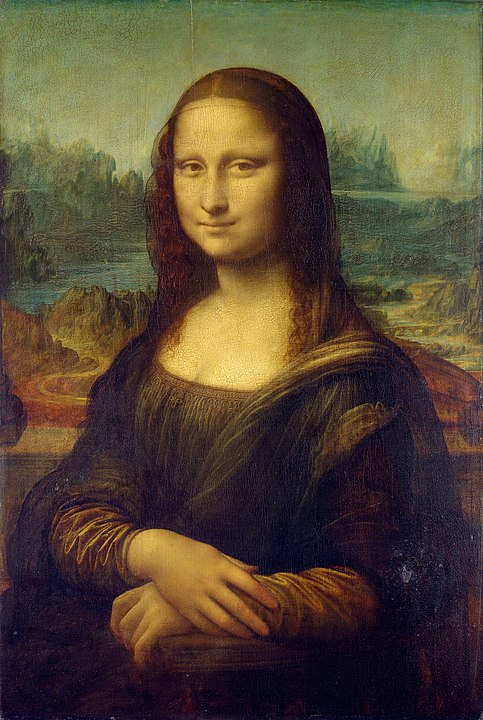
\includegraphics[width=0.3\textwidth]
                    {datas/Mona_Lisa_by_Leonardo_da_Vinci.jpg}
    \caption{La Joconde de Leonard de Vinci}
\end{figure}

%Intro saillance, Irisa et percept
\par
Ce sont l'ensemble de ces éléments qui attirent l'\oe{}il humain qui constituent la saillance. C'est un élément important pour de nombreux domaines. On pense notamment au domaine du marketing et de la publicité qui doivent créer des affiches ou des spots publicitaires avec pour objectif d'attirer le plus possible le regard des consommateurs.

%Intro 
\par
La saillance dans la peinture permet d'analyser et de comprendre le regard humain ainsi que toutes les particularités qui en découlent. L'équipe Percept, équipe de recherche du laboratoire de l'IRISA, se penche sur le sujet et notamment à l'automatisation pour déterminer la saillance dans les peintures à l'aide de modèles de réseaux de neurones basés sur le machine learning.

%Explication du sujet de stage
\par
C'est là que le sujet de mon stage intervient. Cela consiste dans un premier temps à faire l'état de l'art des différents modèles de saillance qui existent sur des images naturelles. Dans un second temps le but est d'adapter le meilleur modèle pour qu'il s'adapte à des peintures. Et enfin à partir des résultats de ce modèle trouver des applications visuelles et ludiques pour montrer l'intérêt d'un tel modèle.

%Explication comment j'ai trouvé le stage et quelles étaient mes motivations
\par 
Ce stage qui m'as été proposé par Olivier Le Meur correspondait à ce que je recherchais. C'est-à-dire un stage basé sur le machine learning, qui fait suite à mon projet industriel à l'ESIR qui consistait à générer des visages au moyen de réseau de neurones antagoniste génératif (GAN). Mais aussi un stage varié qui puisse me permettre de me former sur plusieurs compétences différentes.
% en conclusion : J'ai aimé la liberté et l'autonomie du stage, notamment les discussions qu'on a pu avoir avec Olivier pour déterminer quelles seraient les futur étapes du projet.

\chapter{IRISA}

\par
L'IRISA - Institut de Recherche en Informatique et Systèmes Aléatoires - est
aujourd'hui le plus grand laboratoire de recherche français (+ de 850 personnes)
dans le domaine de l'informatique et des technologies de l'information. Il
couvre l'ensemble des thématiques de ces domaines, de l'architecture des
ordinateurs et des réseaux à l'intelligence artificielle en passant par le génie
logiciel, les systèmes distribués et la réalité virtuelle.

\par
L'IRISA, créé en 1975, est issu d'une volonté de collaboration entre huit établissements tutelles pluridisciplinaires : CentraleSupélec, CNRS, ENS Rennes, IMT Atlantique, Inria, INSA Rennes, Université Bretagne Sud, Université de Rennes 1. Il est aujourd'hui dirigé par Jean Marc Jézéquel.

\begin{figure}[h]
    \centering
    
\includegraphics[width=0.7\linewidth]{datas/logo_irisa.jpg}
    \caption{Logo de l'IRISA}
\end{figure}

\par
l'IRISA est présent sur 3 sites géographiques au sein du territoire breton (Rennes, Lannion et Vannes). Mon stage s'est déroulé dans les locaux de Rennes.
Le laboratoire est structuré en sept départements scientifiques :
\begin{itemize}
    \item D1 - Systèmes Large Échelle
    \item D2 - Réseaux, Télécommunication et Services
    \item D3 - Architecture
    \item D4 - Langage et génie logiciel
    \item D5 - Signaux et Images numériques, Robotique
    \item D6 - Média et interactions
    \item D7 - Gestion des données et dela connaissance
\end{itemize}


\par
L'équipe PERCEPT du département Média et intéractions est spécialisé dans le comportement visuel de différentes populations.

\chapter{Contexte}
% parler de la saillance, fixation, saccades, dataset
\par
Le stage a commencé par de la documentation en rapport avec le sujet de stage. N'ayant pas d'accès à un poste la première semaine de stage, Olivier m'a donné quelques documents introduisant des notions importantes sur le regard humain et la saillance. Ce sont des domaines plutôt liés à l'anatomie et la psychologie mais qu'il est important de comprendre si l'on veut pouvoir interpréter les résultats obtenus en sortie des scripts.
\par
Je vais vous expliquer ici les notions fondamentales qui permettent de comprendre le regard humain et comment il est possible de le mesurer pour l'analyser.

\section{Fixation et saccade}
\label{section:fix_sacc}
\par
Le regard est une alternance entre des périodes où l'\oe{}il reste relativement stationnaire, que l'on appelle "\textbf{fixations}", et de courtes périodes de plus grande mobilité, que l'on appelle "\textbf{saccades}"\cite{gaze}. Ce sont des notions qui ont été décrites pour la première fois en 1879 par Javal et Lamare. Il a été possible d'établir des mesures sur le mouvement des yeux deux décades plus tard (Erdmann et Dodge 1898). Ces mesures ont ouvert le champs aux possibilités d'expérimentation sur la psychologie liée au mouvement des yeux. Cela a permis de mieux comprendre le processus d'analyse quand quelqu'un lit, résoud un problème, regarde un film ou quand quelqu'un regarde une peinture.

\par
Chaque fixation est reliée à une autre fixation par une saccade. Ainsi le regard d'une personne dans le temps est donc constitué d'une succession de fixations et de saccades qui forment une chaine. On appelle cela le \textbf{chemin visuel}. C'est en analysant le chemin visuel que l'on est capable de comprendre comment un individu regarde une peinture ou tout autre élément visuel.

\begin{figure}[!ht]
    \centering
    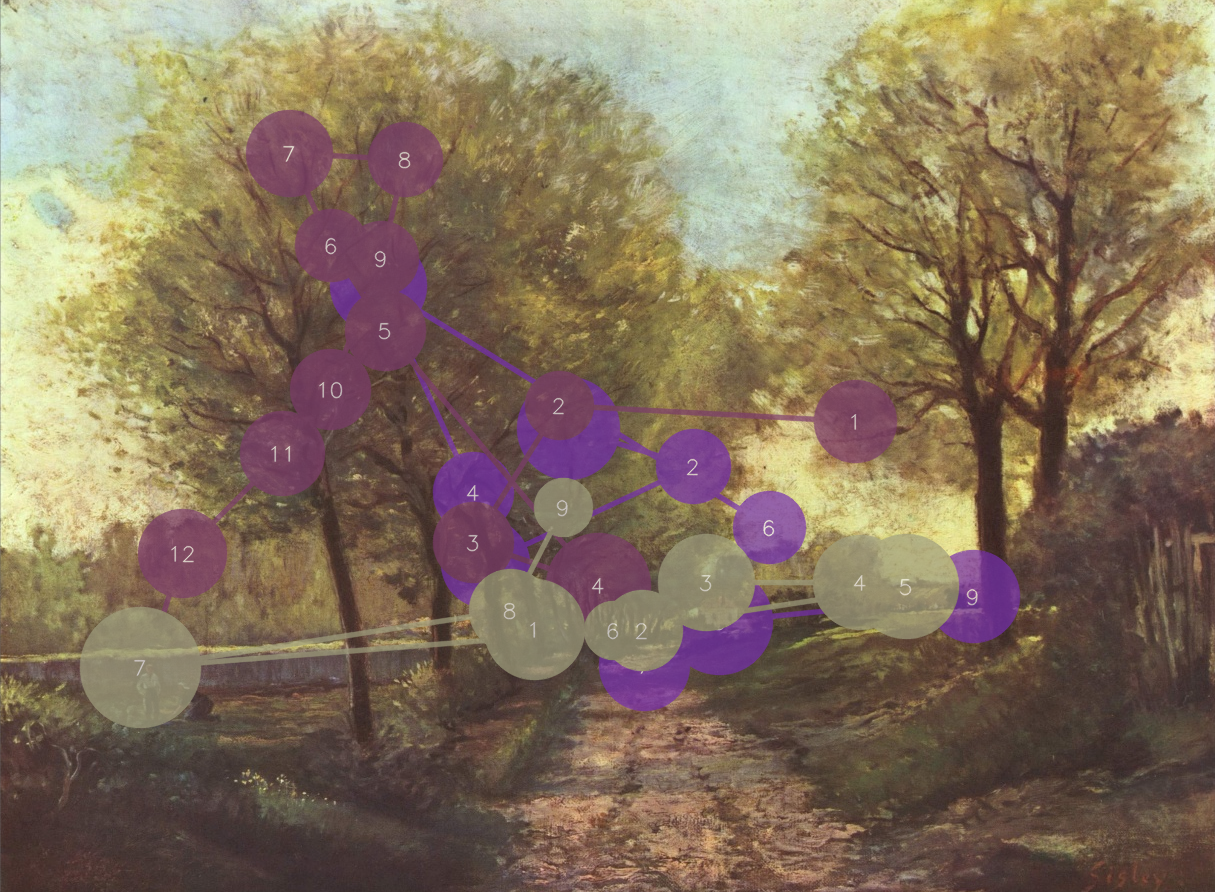
\includegraphics[width=0.7\linewidth]{datas/exemple_scanpaths2.png}
    \caption{Exemple de chemins visuels de 3 observateurs différents}
    \label{ex_scanpath}
\end{figure}

\par
Sur l'image \ref{ex_scanpath} (\emph{Avenue of trees in a small town}, Alfred Sisley, 1866) on peut voir l'exemple d'une représentation de chemins visuels de trois observateurs différents distingués chacun par une couleur différente. Sur cette image chaque fixation est représentée par un cercle numéroté qui correspond à son positionnement dans le parcours du regard. La taille des cercles dépend de la durée de la fixation en question. Ici chaque fixation est reliée à une autre fixation par un trait qui représente une saccade.

\section{Saillance et carte de saillance}
\par
Sur l'exemple précédent il est facile de remarquer que chaque individu aborde la peinture avec un regard différent d'un autre. Cependant il est très important de noter qu'il y a des similarités dans les zones regardées. Il y a des endroits de la peintures que les trois observateurs ont regardé, comme le bout du chemin ou l'arbre de gauche au premier plan, tandis que d'autres endroits sont ignorés, les bordures de la peinture entre autre. Ce sont ces zones plus souvent regardées que l'on appellera des zones saillantes.

\par
La \textbf{saillance} est donc la notion qui définie qu'un élément est facilement remarqué. Elle existe aussi dans le domaine sonore ou linguistique. Ici c'est évidemment la saillance visuelle qui nous intéresse. Un élément dit saillant est donc un élément qui dénote du reste de l'\oe{}uvre et qui attirera le regard de l'observateur. Les critères qui définissent la saillance d'un objet sont régies par deux facteurs important. Le facteur "\textbf{Bottom-up}" basé sur les information simple comme les couleurs, le contraste ou la luminosité. Le facteur "\textbf{Top-down}" lui est basé sur des informations propres à l'observateur. Il peut être influencé par une tâche à accomplir, par sa culture, ses connaissances, son âge...\ C'est à partir de tous ces éléments que l'on peut déduire une forte connexion entre le mouvement des yeux, ou le chemin visuel, et la saillance d'une peinture.

\par
De cette relation on va pouvoir, à partir du chemin visuel de plusieurs observateurs, générer une \textbf{carte de saillance} (voir image \ref{ex_saliency_map}). Celle-ci va nous permettre de mettre en évidence les éléments saillants d'une image. Elle est obtenue en moyennant les points de fixations de différents observateurs. Plus une zone est blanche, plus elle est saillante.

\begin{figure}[!ht]
    \centering
    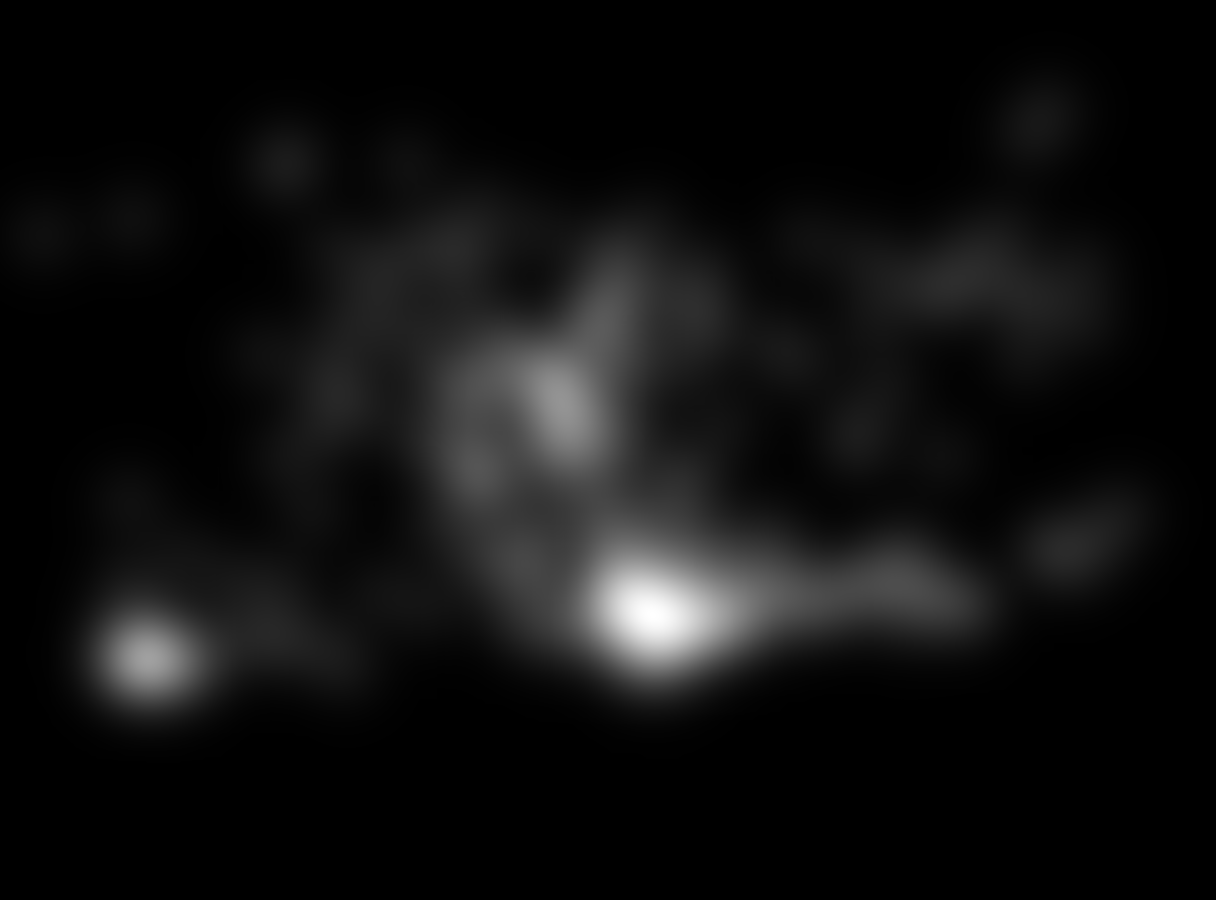
\includegraphics[width=0.7\linewidth]{datas/exemple_saliency_map.png}
    \caption{Exemple de carte de saillance}
    \label{ex_saliency_map}
\end{figure}

\par
Si on superpose la carte de saillance et la peinture associée on peut facilement voir quels sont les éléments saillants de l'\oe{}uvre (voir image \ref{saliency_map_transparency}). Ici la carte de saillance nous révèle que le village au bout du chemin, les deux personnages en bas à gauche et la végétation au premier plan sont les éléments saillants de l'\oe{}uvre.

\begin{figure}[!ht]
    \centering
    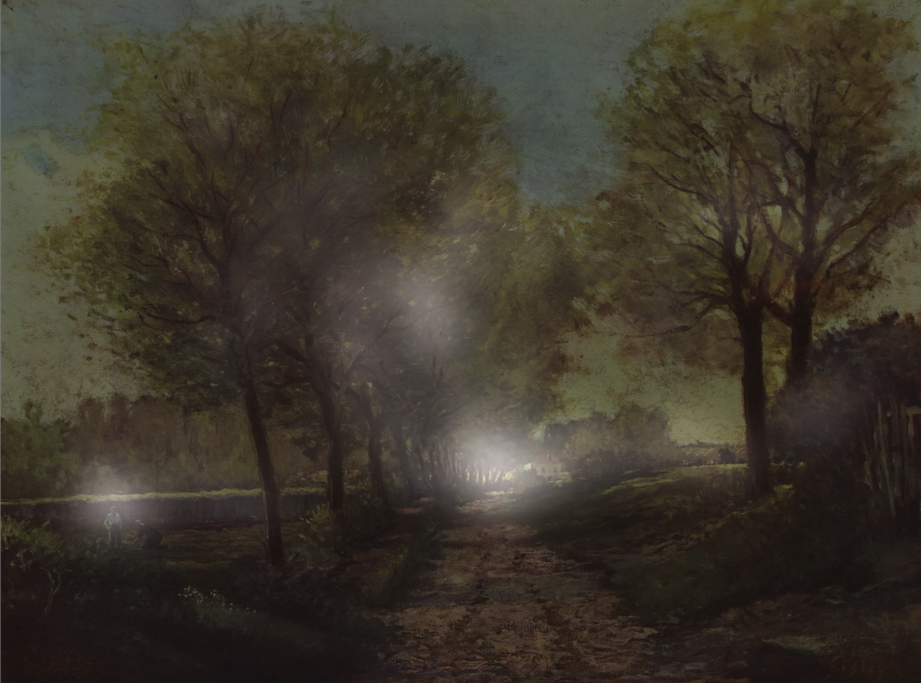
\includegraphics[width=0.7\linewidth]{datas/exemple_saliency_map_transparency.png}
    \caption{Carte de saillance et peinture superposées}
    \label{saliency_map_transparency}
\end{figure}

\par
Mon but lors de ce stage sera d'entrainer un réseau de neurones capable de générer une carte de saillance avec comme seule entrée une peinture. 

\section{Base de données et oculométrie}
\label{database}
\par
Afin de pouvoir entrainer un réseau de neurones il nous faut une base de données avec des données oculométriques sur des peintures. C'est-à-dire une base de données avec l'enregistrement du chemin visuel de différents observateurs qui regardent une peinture.

\par
La mesure du mouvement des yeux d'une personne est possible grâce à un \textbf{oculomètre} (voir image \ref{oculo}). Cet appareil retranscrit le regard d'un observateur avec une grande précision et peut nous donner des informations comme la position et la durée d'une fixation. Inventé vers la fin du 19\up{ème} siècle, il en existe aujourd'hui des versions électroniques très efficace.

\begin{figure}[!ht]
    \centering
    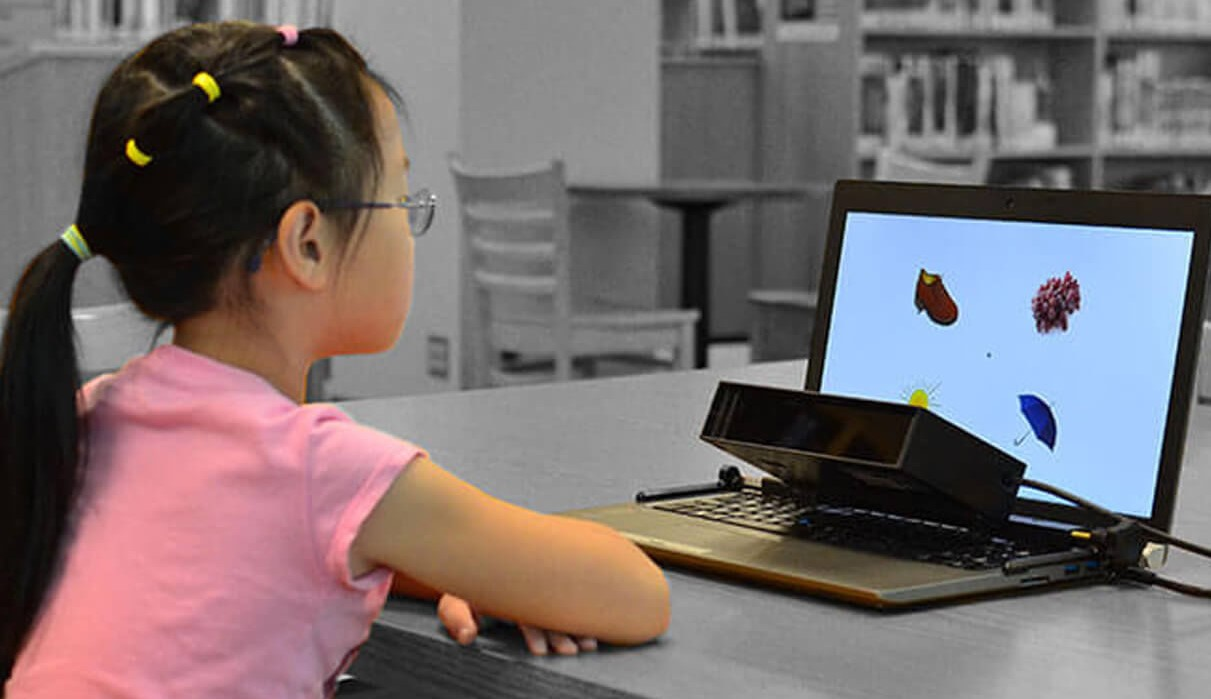
\includegraphics[width=0.7\linewidth]{datas/oculometre.jpg}
    \caption{Exemple d'oculomètre}
    \label{oculo}
\end{figure}

Des étudiants de l'ISTIC ont effectué un stage sous la direction d'Olivier Le Meur pour constituer une base de données oculométrique de 21 observateurs sur un total de \textbf{150 peintures}. Ce sont des peintures de 5 grands mouvements artistiques (Fauvisme, Impressionnisme, Réalisme, Romantisme et Pointillisme) avec chacun 3 genres (Nature morte, Nu, Paysage). Chaque participant avait 5 secondes pour regarder une peinture ce qui nous donne des données oculométrique étaler de 5 secondes dans le temps.

\chapter{Présentation et premiers programmes}

\section{Présentation de la journée du patrimoine de l'IRISA}

\par
Olivier m'a proposé de réaliser un diaporama pour le stand de l'équipe Percept lors de la journée du patrimoine à l'IRISA programmé le 24 Mars 2020 à l'origine mais qui a été reportée à cause du contexte actuel de situation sanitaire d'urgence. J'ai tout de même réalisé la présentation et devrait être diffusée à la prochaine journée du patrimoine. Olivier m'as conseillé de réaliser le diaporama en \LaTeX{} qui est un langage de programmation qui permet de réaliser des documents équivalents à ceux édités sous Word ou Open Office. L'avantage de ce langage est qu'il permet d'automatiser beaucoup d'élément, notamment la mise en page. Dans ma présentation je devais mettre une dizaine d'\oe{}uvres avec pour chacune d'elle une bonne quantité d'information (description, carte de saillance...). \LaTeX{} m'a permis d'automatiser la mise en diapositive des peintures pour un rendu de qualité.

\begin{figure}[!ht]
    \centering
    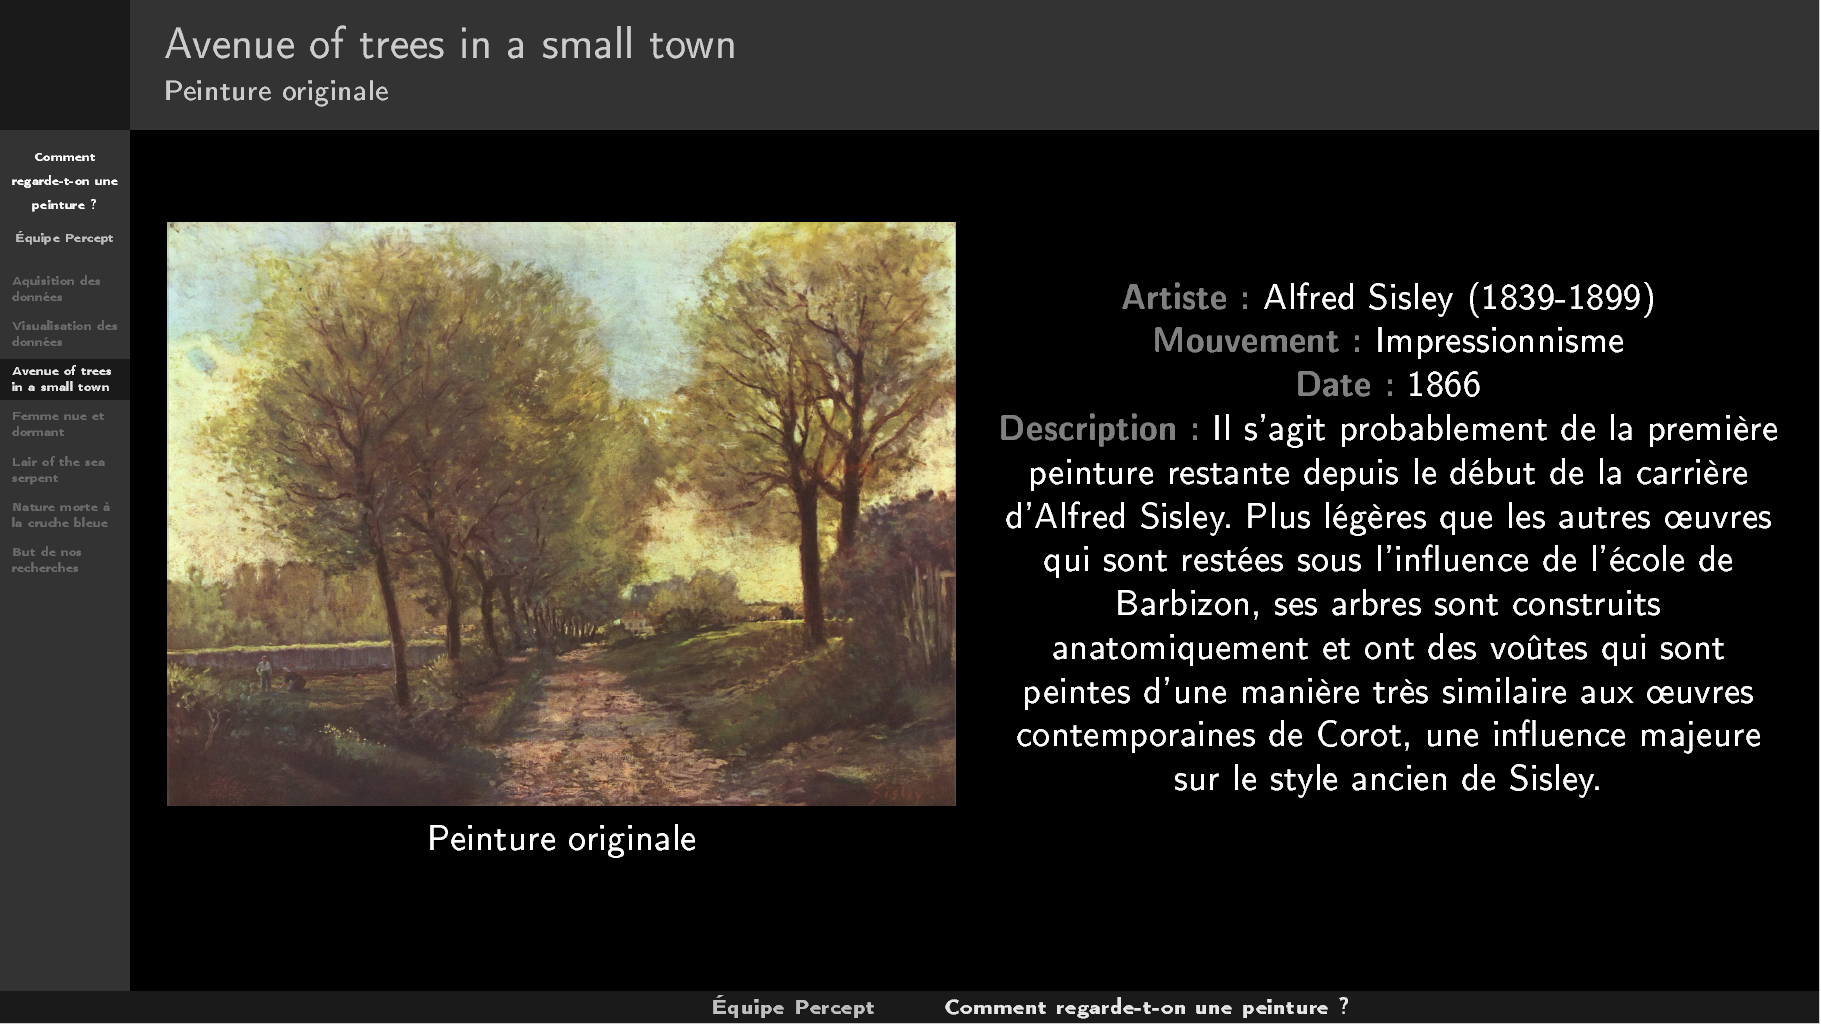
\includegraphics[width=0.7\linewidth]{datas/exemple_diapo.png}
    \caption{Extrait de la présentation}
    \label{ex_diapo}
\end{figure}

\par
Afin de rajouter des animations dans mon diaporama, notamment des vidéos pour faciliter la compréhension, je me suis lancé dans la programmation de petits programmes en langage Python. Même si il y a eu de nombreux TPs en Python lors de cette année à l'ESIR j'ai remarqué que j'avais encore beaucoup à apprendre en regardant ce qu'il se faisait déjà sur le gitlab de l'équipe Percept (site web qui permet d'échanger et de sauvegarder facilement des documents). Cela m'a aussi permis de me familiariser avec les différentes données présentes dans la base de données oculométrique.

\section{Vidéo fondue}

Le premier script permet de créer une vidéo avec une transition en fondu entre chaque image donnée en entrée du programme. L'intérêt d'un tel script est de le combiner au résultat d'un autre programme du gitlab qui donnait des cartes de chaleur de saillance. Ce sont des cartes de saillance en couleur où les zones saillantes sont représentées par des couleurs chaudes. Cela permet de faire évoluer la carte de chaleur de saillance en fonction du temps d'observation (voir Image \ref{fondu}). Pour ma présentation j'ai généré des cartes de chaleur au bout de 1 seconde d'observation, puis au bout de 2, etc. jusqu'à 5 secondes d'observation. La vidéo permettait donc d'enchainer les différentes cartes de chaleur avec un rendu propre avec pour but final d'analyser comment la saillance évoluait au cours du temps.

\begin{figure}[!ht]
    \centering
    \begin{subfigure}{.3\textwidth}
        \centering
        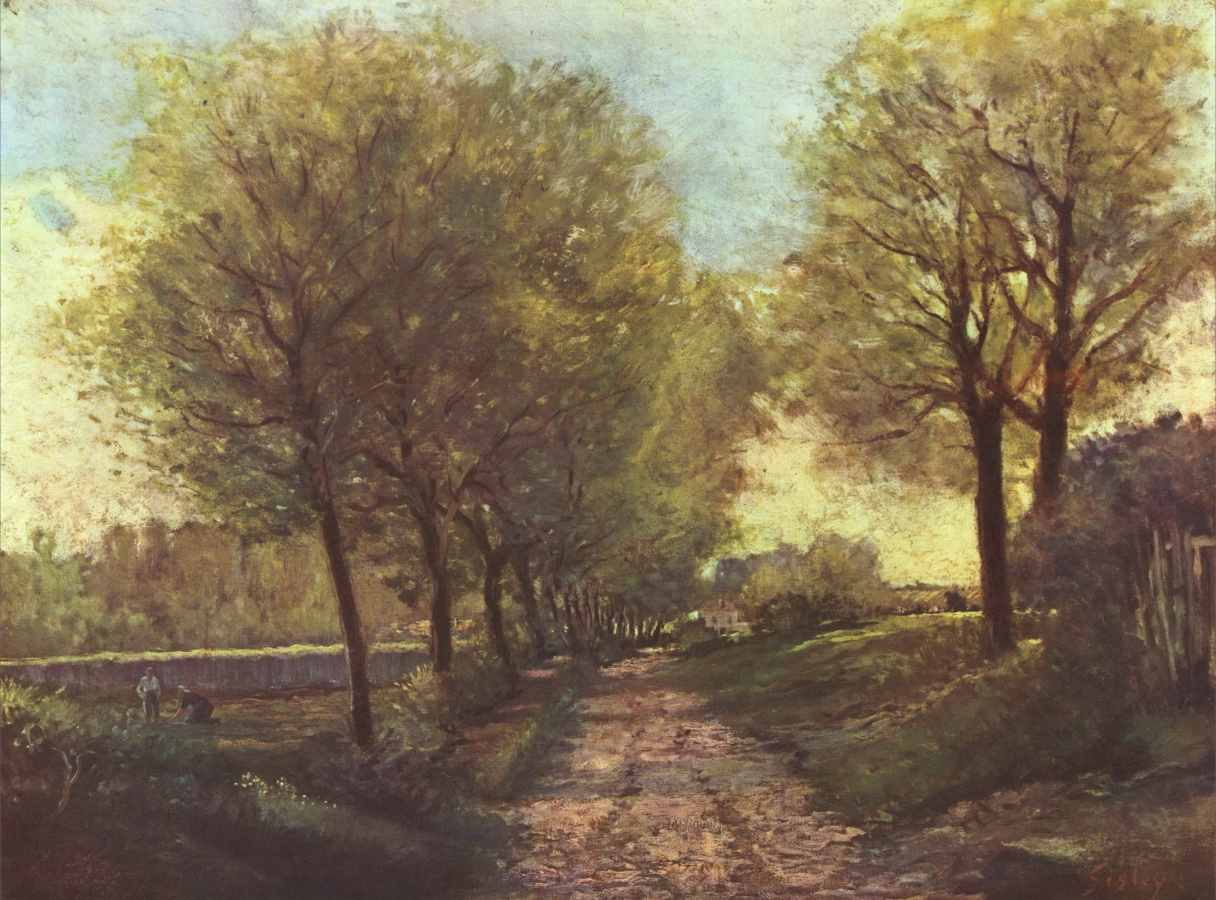
\includegraphics[width=\linewidth]{datas/fondu_00.jpg}
        \caption{}
    \end{subfigure}
    \begin{subfigure}{.3\textwidth}
        \centering
        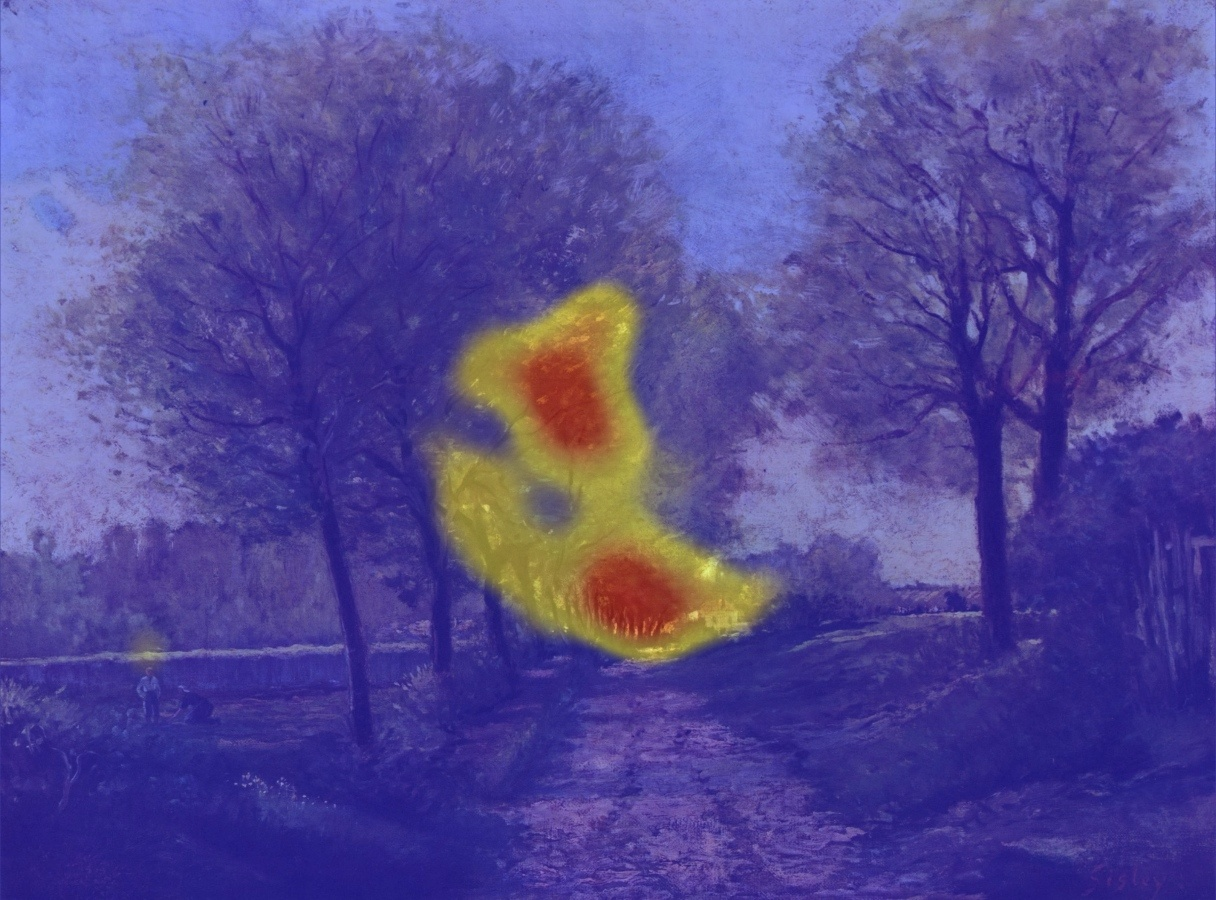
\includegraphics[width=\linewidth]{datas/fondu_02.jpg}
        \caption{}
    \end{subfigure}
    \begin{subfigure}{.3\textwidth}
        \centering
        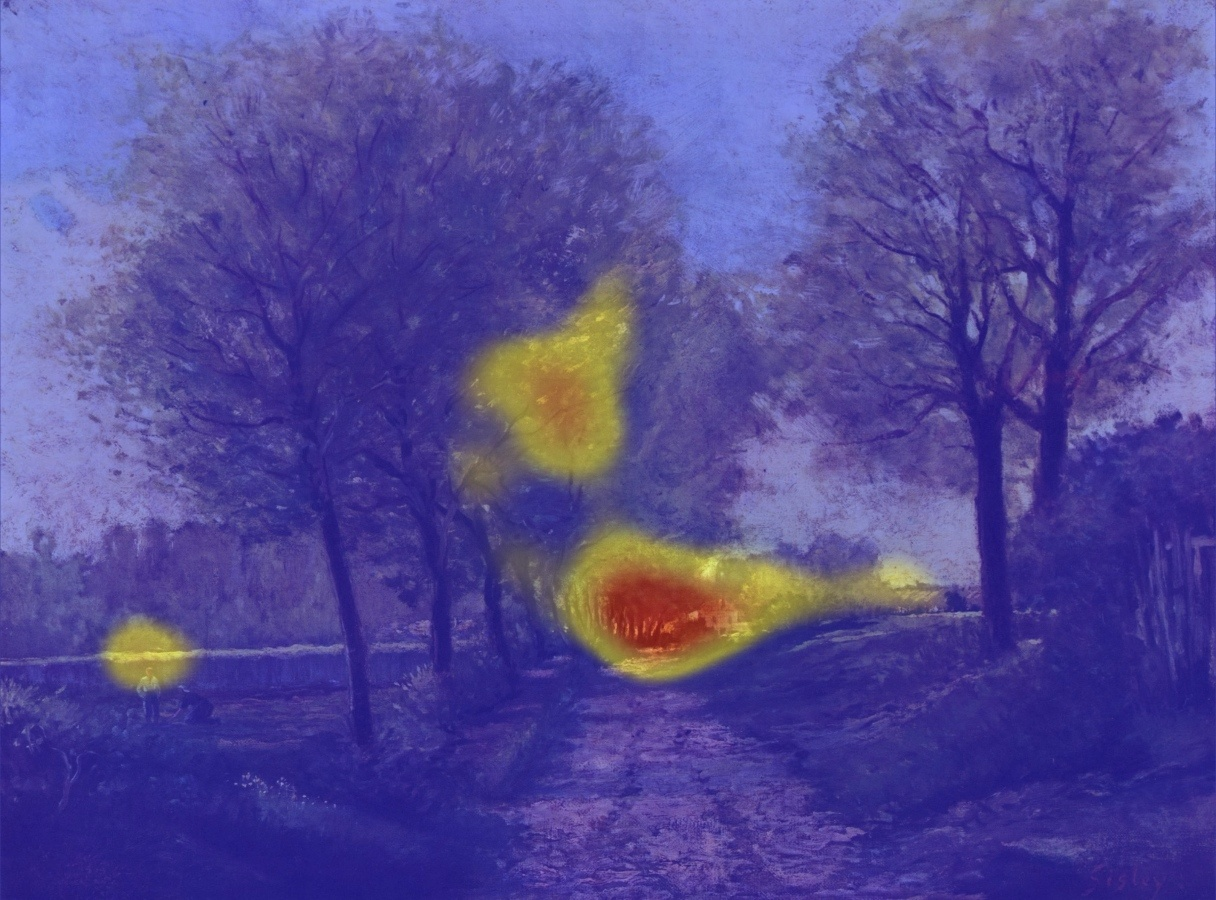
\includegraphics[width=\linewidth]{datas/fondu_05.jpg}
        \caption{}
    \end{subfigure}
    \caption{(a) Peinture originale, (b) Carte de chaleur de saillance après 2s d'observation, (c) Carte de chaleur de saillance après 5s d'observation}
    \label{fondu}
\end{figure}

\par
Ce programme n'est pas très compliqué en soit mais il m'a permis de découvrir des librairies sur Python très utiles que je n'avais jamais essayé auparavant.

\section{Vidéo chemins visuels}

Mon deuxième script consistait à afficher les chemins visuels avec la réprésentation avec des cercles et des lignes vu précédemment avec l'image \ref{ex_scanpath}. Cela permet de visualiser le mouvement des yeux de l'observateur et de pouvoir suivre son regard. L'inconvénient de ce programme c'est qu'avec plusieurs observateurs l'image était rapidement surchargée et les couleurs choisies aléatoirement pour différencier les différents observateurs peuvent êtres très similaires.

\par
J'ai donc fait évoluer ce script en y ajoutant de l'animation. J'ai rajouté une option qui permettait de générer une vidéo où chaque cercle (donc chaque fixation) s'affichait les uns après les autres. Cela permet donc d'avoir à la fin de vidéo toujours une image surchargée mais comme le spectateur a suivi le déroulement de l'animation, celui-ci est beaucoup moins confus. Ce point est aussi vrai pour l'inconvénient des couleurs trop similaires.

\chapter{Modèles de saillance}

\section{État de l'art et choix du modèle de saillance}

\par
Il existe aujourd'hui de nombreux modèles de saillance qui permettent de générer des cartes de saillance à partir de scènes naturelles (photos). Ces programmes donnent des résultats plus ou moins proches de la vérité terrain sans pour autant réellement l'atteindre. En revanche le gros avantage est qu'ils permettent d'éviter la fastidieuse tâche de récupération des données oculométriques sur des humains tout en ayant des résultats satisfaisant.

\par
Il y a aujourd'hui deux types de modèles de saillance : les modèles "fait-main" qui appliquent des traitements sur l'image suivant des fonctions mathématiques et les modèles basés sur l'apprentissage profond qui s'entrainent sur des bases de données pour s'améliorer. Les modèles fait-main sont en général plus anciens et précèdent l'avènement du machine learning et de l'apprentissage profond. Ils sont donc généralement moins puissants que les modèles profonds.

\par
Ici notre objectif est de déterminer parmis les modèles qui existent quel est le modèle qui obtient les meilleurs résultats quand on lui donne des peintures en entrée. Pour pouvoir comparer le plus objectivement possible les résultats, il est nécessaire d'utiliser des métriques de qualité. Comme le mètre est utilisé pour mesurer une distance, les métriques sont des outils de mesure avec des échelles variées qui permettent d'associer un score jugeant la qualité de nos cartes de saillances. Il est préférable d'utiliser plusieurs métriques différentes puisque chacune d'entre elles à ses qualités et ses défauts. Ici les métriques utilisées sont celles du benchmark du MIT \cite{benchmark_MIT}.

\par
Mon rôle ici a été de tester tous les modèles profonds pour vérifier dans un premier temps s'il était possible de les faire tourner et dans un second temps de données des peintures en entrées pour pouvoir y appliquer les métriques de qualité. On peut voir dans l'image \ref{fig:saliencyModel} les résultats des différents modèles comparés à la carte de saillance originale. 

\par
Visuellement il est assez évident de dire que les modèles profonds sont plus proche de l'original que les autres. Cela se confirme dans l'analyse des métriques. Dans le tableau \ref{tab:scores} on voit que les scores moyens des modèles fait-mains sont tout le temps moins bons que les modèles profonds. Les scores en gras sont les meilleurs scores entre tout les modèles. Ici SAM-ResNet est clairement le plus performant avec le meileur score dans cinq des sept métriques utilisées. C'est logiquement qu'avec Olivier on a choisi de continuer nos recherches avec SAM-ResNet.

\vfill

\begin{figure}[ht]
    \centering
    \begin{subfigure}{0.24\textwidth}
        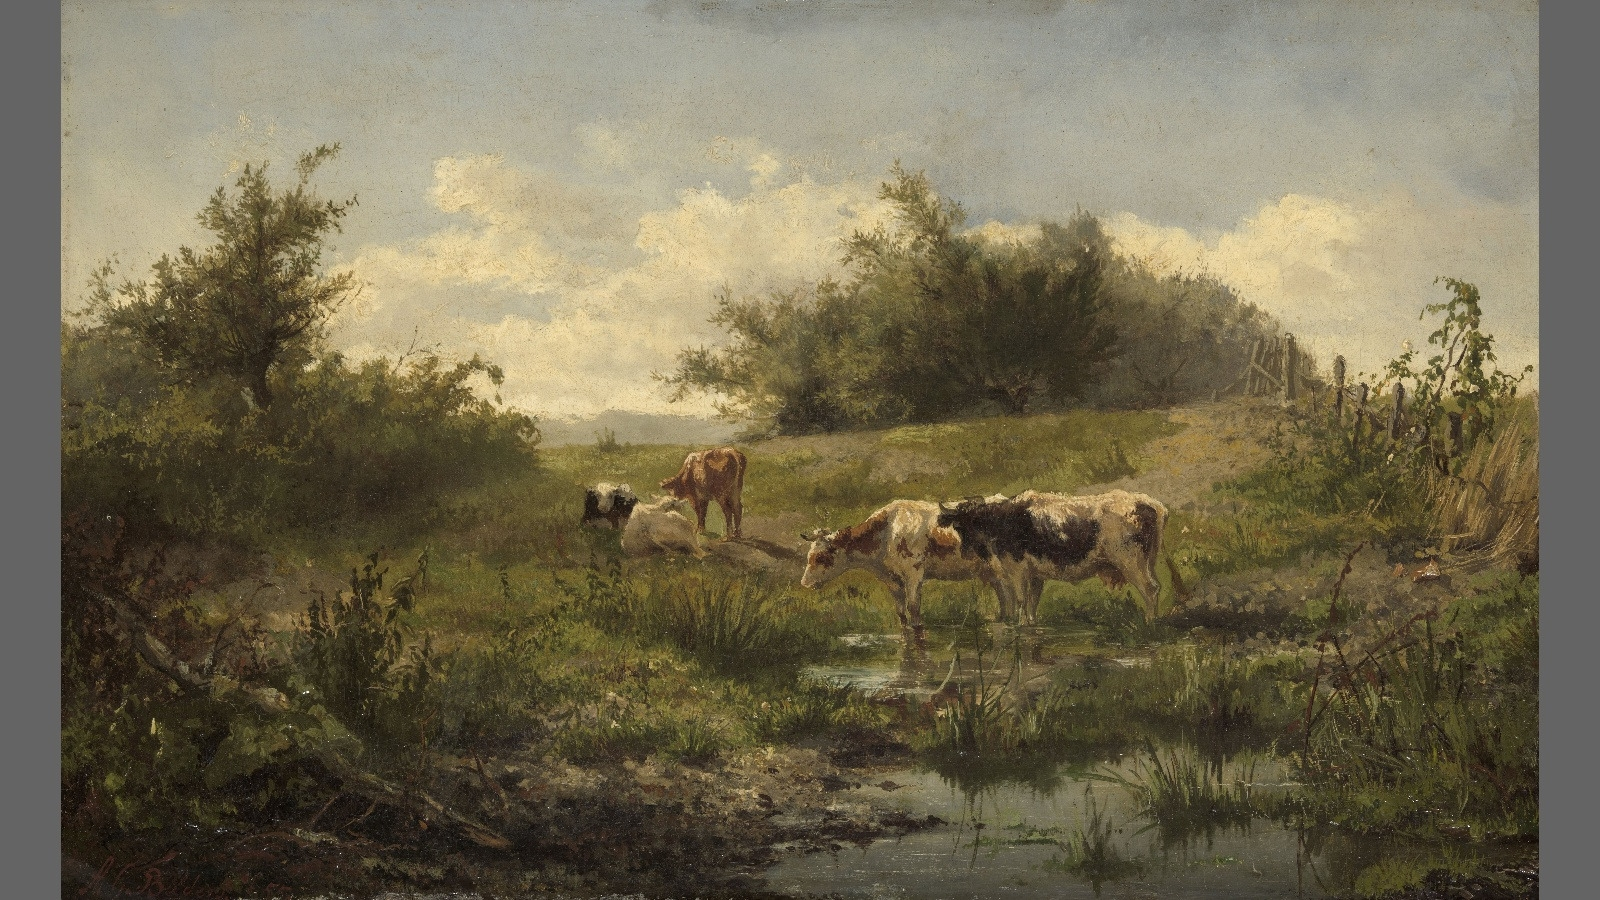
\includegraphics[width=\linewidth]{datas/predictions/stimulus_cows_at_a_pond_Bilders_1856.jpg}
        \caption{}
    \end{subfigure}
    \begin{subfigure}{0.24\textwidth}
        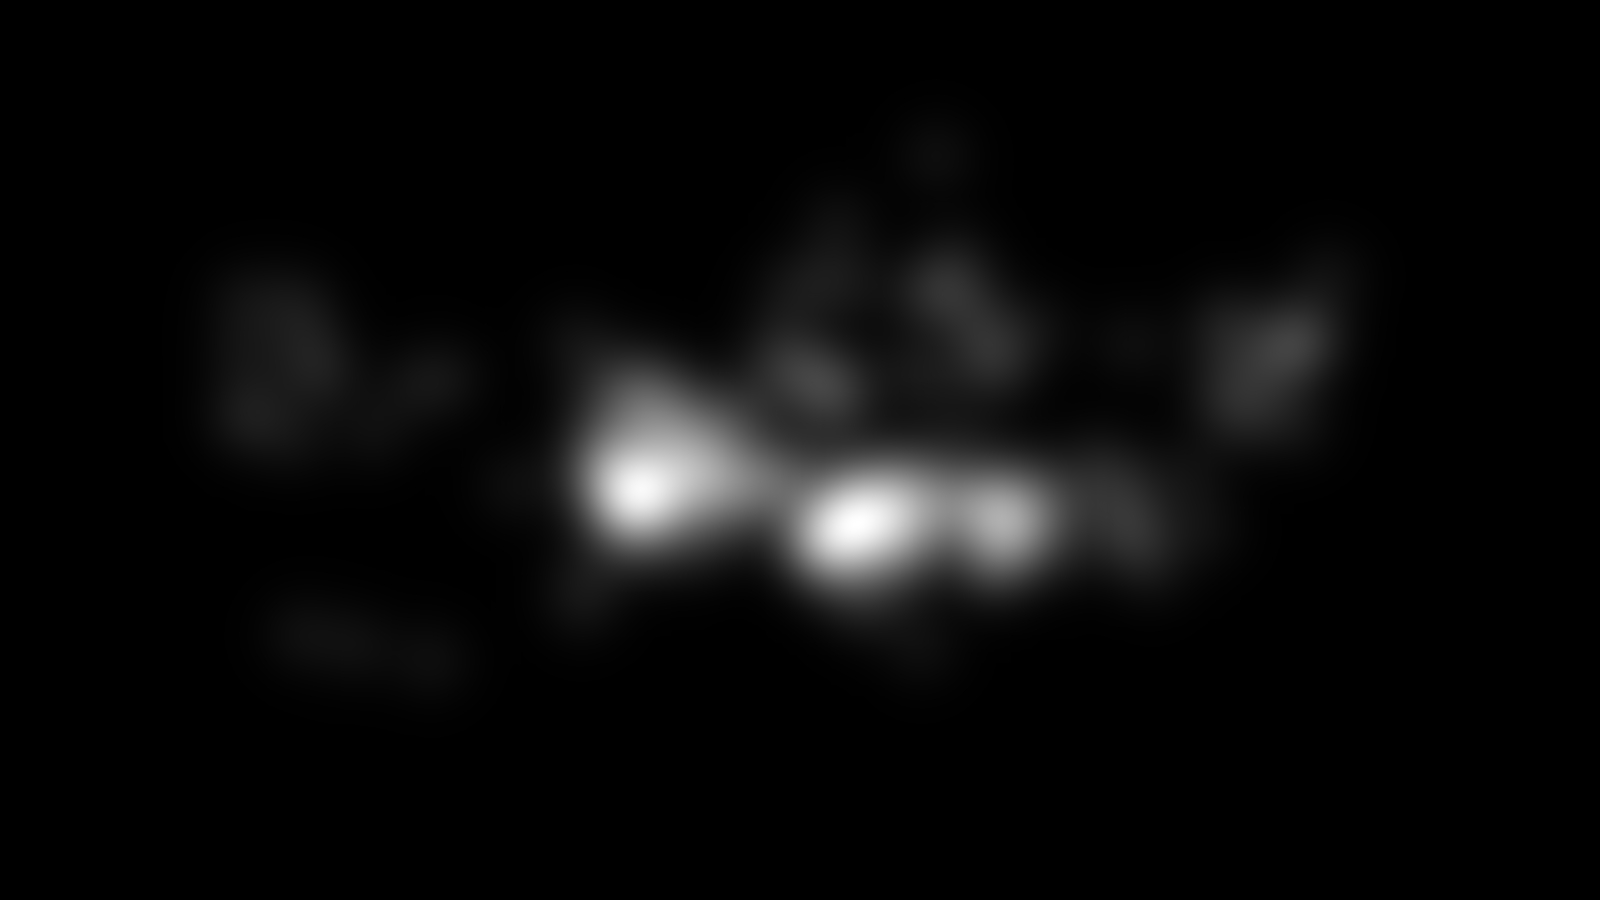
\includegraphics[width=\linewidth]{datas/predictions/human_cows_at_a_pond_Bilders_1856.jpg}
        \caption{}
    \end{subfigure}

    \begin{subfigure}{0.24\textwidth}
        \includegraphics[width=\linewidth]{datas/predictions/gbvs_cows_at_a_pond_Bilders_1856.jpg}
        \caption{GBVS}
    \end{subfigure}
    \begin{subfigure}{0.24\textwidth}
        \includegraphics[width=\linewidth]{datas/predictions/aws_cows_at_a_pond_Bilders_1856.jpg}
        \caption{AWS}
    \end{subfigure}
    \begin{subfigure}{0.24\textwidth}
        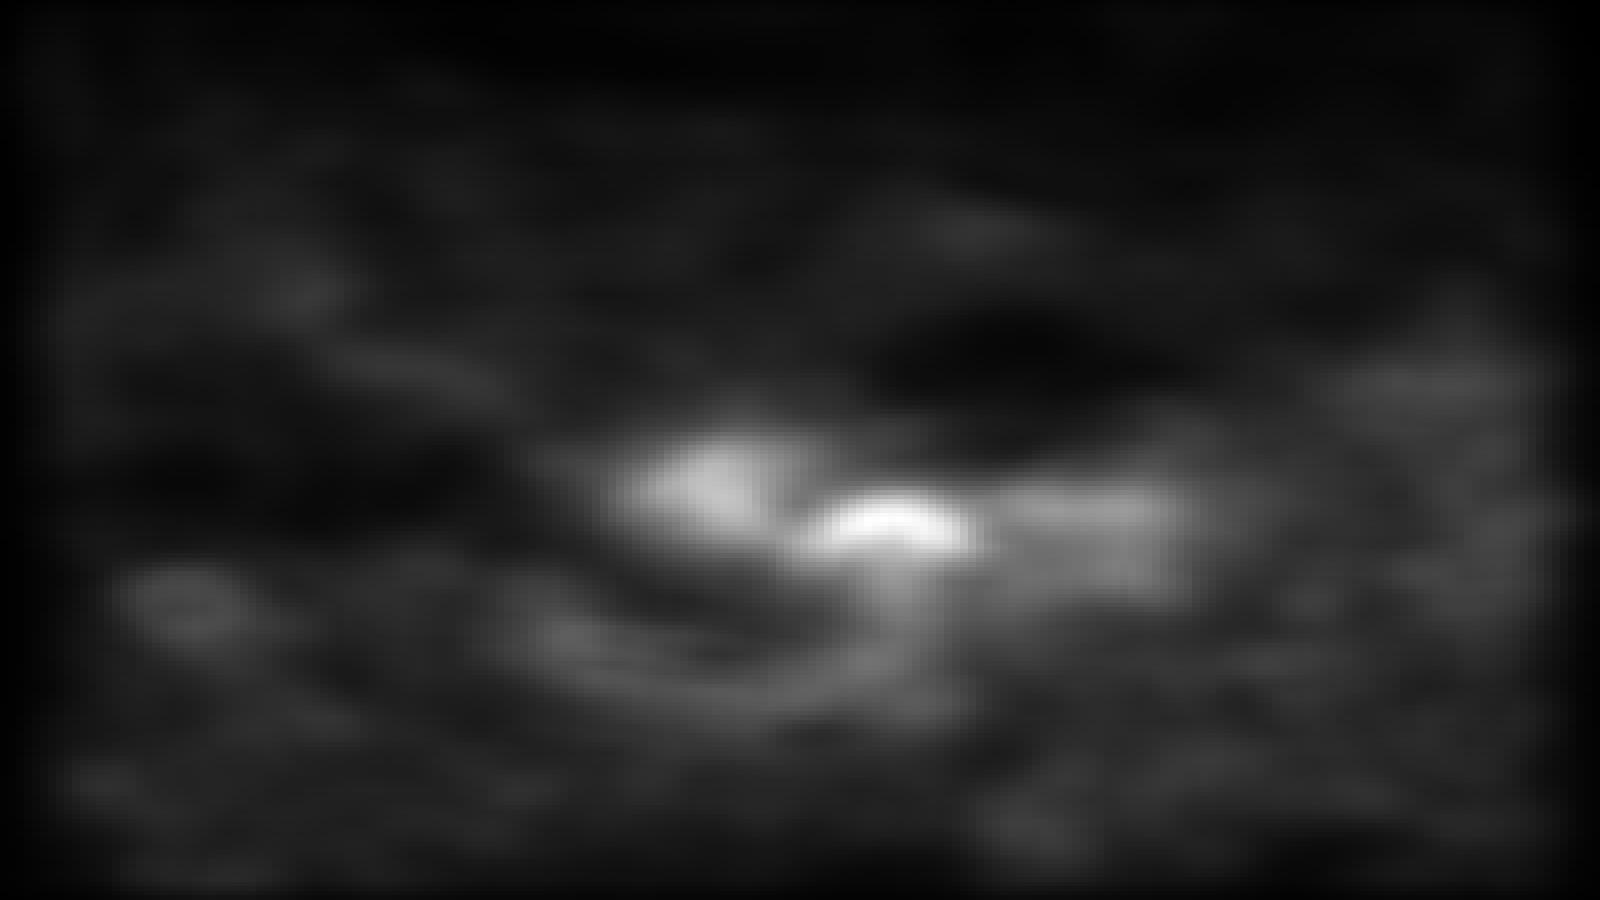
\includegraphics[width=\linewidth]{datas/predictions/rare2012_cows_at_a_pond_Bilders_1856.jpg}
        \caption{RARE2012}
    \end{subfigure}
    \begin{subfigure}{0.24\textwidth}
        \includegraphics[width=\linewidth]{datas/predictions/aim_cows_at_a_pond_Bilders_1856.jpg}
        \caption{AIM}
    \end{subfigure}

    \begin{subfigure}{0.24\textwidth}
        \includegraphics[width=\linewidth]{datas/predictions/mlnet_cows_at_a_pond_Bilders_1856.jpg}
        \caption{MLNET}
    \end{subfigure}
    \begin{subfigure}{0.24\textwidth}
        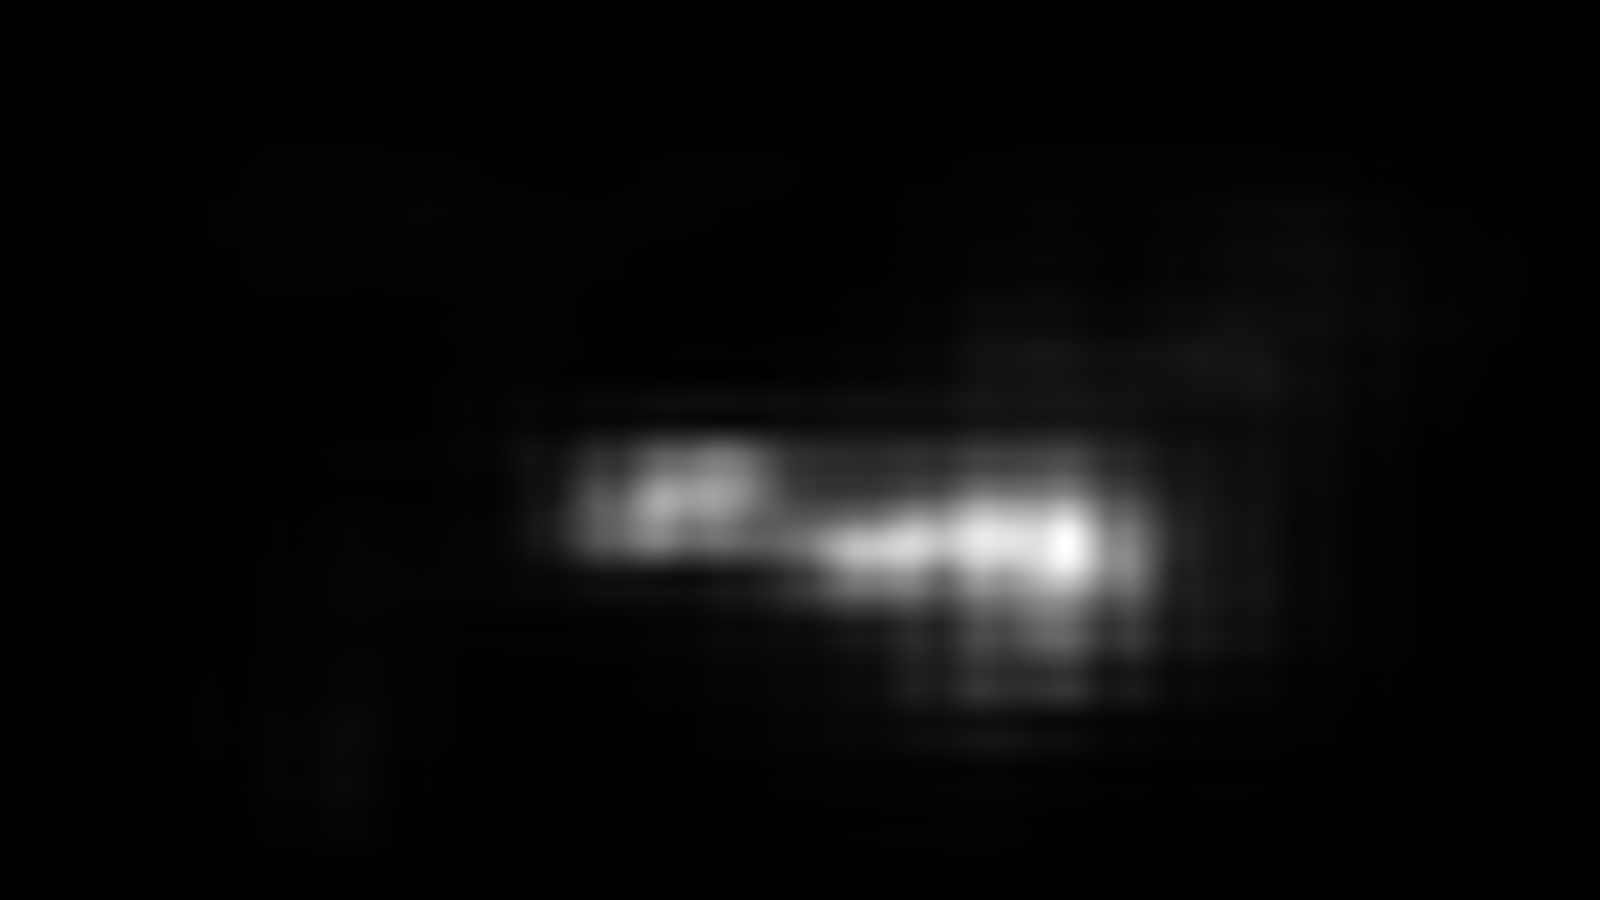
\includegraphics[width=\linewidth]{datas/predictions/SALICON_cows_at_a_pond_Bilders_1856.jpg}
        \caption{SALICON}
    \end{subfigure}
    \begin{subfigure}{0.24\textwidth}
        \includegraphics[width=\linewidth]{datas/predictions/sam_vgg_cows_at_a_pond_Bilders_1856.jpg}
        \caption{SAM-VGG}
    \end{subfigure}
    \begin{subfigure}{0.24\textwidth}
        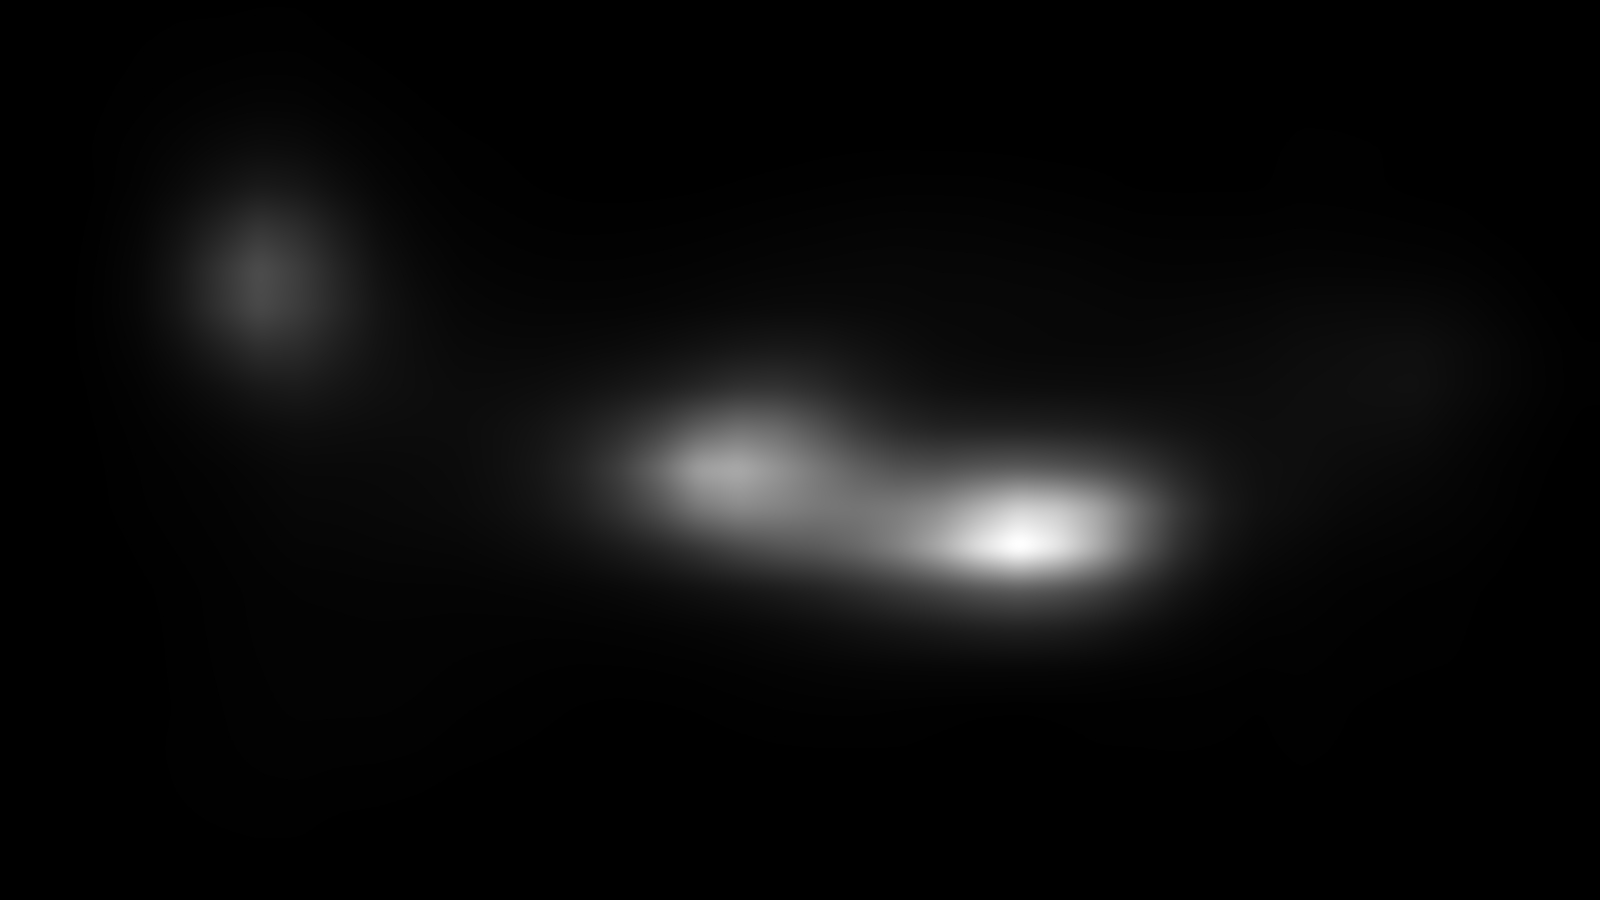
\includegraphics[width=\linewidth]{datas/predictions/sam_resnet_cows_at_a_pond_Bilders_1856.jpg}
        \caption{SAM-ResNet}
    \end{subfigure}
     
    \caption{Cartes de saillance de modèles fait-mains (2\up{ème} ligne) et profonds (3\up{ème} ligne). La 1\up{ère} ligne illustre le stimuli originale et sa carte de saillance humaine}
    \label{fig:saliencyModel}
\end{figure}

\vfill

\begin{table}[ht]
    \centering
        \begin{tabular}{|l|l|l|l|l|l|l|}
		\hline
        Modèle & CC~$\uparrow$ & KL~$\downarrow$ & SIM~$\uparrow$ & NSS~$\uparrow$ & AUC-B~$\uparrow$ & AUC-J~$\uparrow$\\
		\hline
        GBVS        & 0.506 & 0.962 & 0.446 & 1.256 & \textbf{0.809} & 0.817\\
        RARE2012    & 0.443 & 1.020 & 0.438 & 1.103 & 0.777 & 0.786\\
        AIM         & 0.315 & 1.245 & 0.371 & 0.772 & 0.723 & 0.735\\
        AWS         & 0.427 & 1.045 & 0.430 & 1.083 & 0.762 & 0.769\\
		\hline
        Moyenne     & 0.422 & 1.068 & 0.421 & 1.053 & 0.774 & 0.776\\
		\hline
        MLNET       & 0.576 & \textbf{0.832} & 0.513 & 1.524 & 0.770 & 0.818\\
        DeepGazeII  & 0.485 & 0.896 & 0.488 & 1.394 & 0.679 & 0.804\\
        SALICON     & 0.538 & 0.880 & 0.517 & 1.445 & 0.708 & 0.827\\
        SAM ResNet  & \textbf{0.700} & 0.984 & \textbf{0.613} & \textbf{1.834} & 0.782 & \textbf{0.862}\\
        SAM VGG     & 0.617 & 0.970 & 0.561 & 1.603 & 0.752 & 0.846\\
		\hline
        Moyenne     & 0.583 & 0.912 & 0.551 & 1.560 & 0.738 & 0.831\\
		\hline
        \end{tabular}
    \caption{Performances des modèles de saillance sur les peintures de la base de données.}
    \label{tab:scores}
\end{table}

\vfill

% \newpage
\section{Entrainement du modèle}


\chapter{Applications}

\section{Effet Ken burns/Ken Moore}

\chapter{Conclusion}

Au cours de ces 6 mois de stage au sein de l'IRISA et plus particulièrement l'équipe Percept, j'ai pu découvrir le monde de la recherche. Une expérience unique qui m'as permis de me faire une idée de ce qui m'attend si je me lance dans le développement d'une thèse.

J'ai aussi pu découvrir le domaine de la saillance. Je pense que pour un étudiant qui a pour but de travailler dans l'imagerie numérique il est important de savoir coment fonctionne le regard humain. On a bien sûr déjà eu des cours sur ce sujet à l'ESIR mais ici j'ai pu approfondir mes connaissances sur ce sujet.

J'ai beaucoup aimé l'échange qu'il y a entre les différentes personnes au sein de l'équipe. Dès mon arrivée je me suis senti intégré a ce groupe de travail. Je l'ai aussi ressenti lors des réunions où tous les membres de l'équipe devaient présenter leur projet moi y compris. C'est un très bon moyen de comprendre ce que font les collègues et à l'inverse expliquer mon sujet. Cela permet donc par la suite que chacun puisse proposer des idées ou des solutions aux problèmes d'autres personnes qui bloquent dans leur projet.

J'ai beaucoup appris en programmation et particulièrement en Python et en \LaTeX. Pour Python je n'avais jamais réalisé de projet aussi concret et qui soit ensuite mise à la disposition de l'équipe. \LaTeX\ est un langage que j'ai eu la chance d'avoir le temps de maitriser suffisament pour obtenir des documents sobres, professionnels et automatiques.

Ce fut aussi intéressant de travailler avec l'apprentissage profond qui est aujourd'hui présent partout. Même si j'avais déjà travaillé sur un projet de machine learning à l'ESIR, j'ai pu renforcé mes connaissances sur le sujet étant donné qu'il est vraiment vaste.

\bibliographystyle{plain}
\addcontentsline{toc}{chapter}{Bibliographie}
\begin{thebibliography}{99}

	\bibitem{irisa}
	  Site de l'IRISA - Présentation du laboratoire\\
      \link{https://www.irisa.fr/fr/page/recherche-innovation-sciences-technologies-du-numerique}
      
      \bibitem{percept}
	  Site de l'IRISA - Présentation de l'équipe PERCEPT\\
      \link{https://www.irisa.fr/fr/equipes/percept}

      \bibitem{gaze}
      \emph{Art, Aesthetics, and the brain}, 2015\\
      par J.P. Huston, M. Nadal, F. Mora, L.F. Agnati et C.J. Cela-Conde

      \bibitem{benchmark_MIT}
      \emph{Mit saliency benchmark}, 2015\\
      par Bylinskii Z, Judd T, Borji A, Itti L, Durand F, Oliva A, et al.

\end{thebibliography}


\appendix
\addcontentsline{toc}{chapter}{Annexes}
\chapter*{Annexes}




\end{document}

% Plan :
% Page de garde -- Done
% Remerciements -- Done
% Résumé (anglais français) -- Done
% Sommaire -- Done
% Introduction
%%% rapide résumé contexte, entreprise, explication du sujet et pk avoir choisi le stage
% Présentaion Irisa et mission de stage
% Analyse du problème et de son contexte / étude de l'existant / méthode et plan de travail
%%% Introduction à la saillance et au machine learning
% Solution proposée / Travail réalisé / Résultats développés
%%% prise en main de python et de la saillance : video fondu et scanpath
%%% diapo pour journée du patrimoine irisa
%%% puis benchmark des differents algo
%%% puis finetuning de SAM-RESNET (the best)
%%% appli : ken burns video + ...
% évaluation / Interprétation des résultats / Retour d'expérience / Bilan
%%% finetuning a permis de faire un papier (accepter par plosone ?)
% Conclusion
% Biblio
% Annexes


